\chapter{$H_0$ and the different anchor distances}
\label{appendix1-h0}

\section{Introduction}

We have seen in Section \ref{chapter-h0:Summary} that results including all the available distance anchors are robust against the statistical method utilised in the analysis. In order to better understand both the data sets and the results in our 'standard analysis' we investigate below the application of our method to different combination of distance anchors excluding one or two of them. Our preferred $H_0$ measurements from subsections \ref{Subsection:A-NGC4258}-\ref{Subsection-A-Combining-distance-anchors} are shown in Figure \ref{Fig:single-combined-anchor}. 

\begin{figure}[hbtp]
\centering
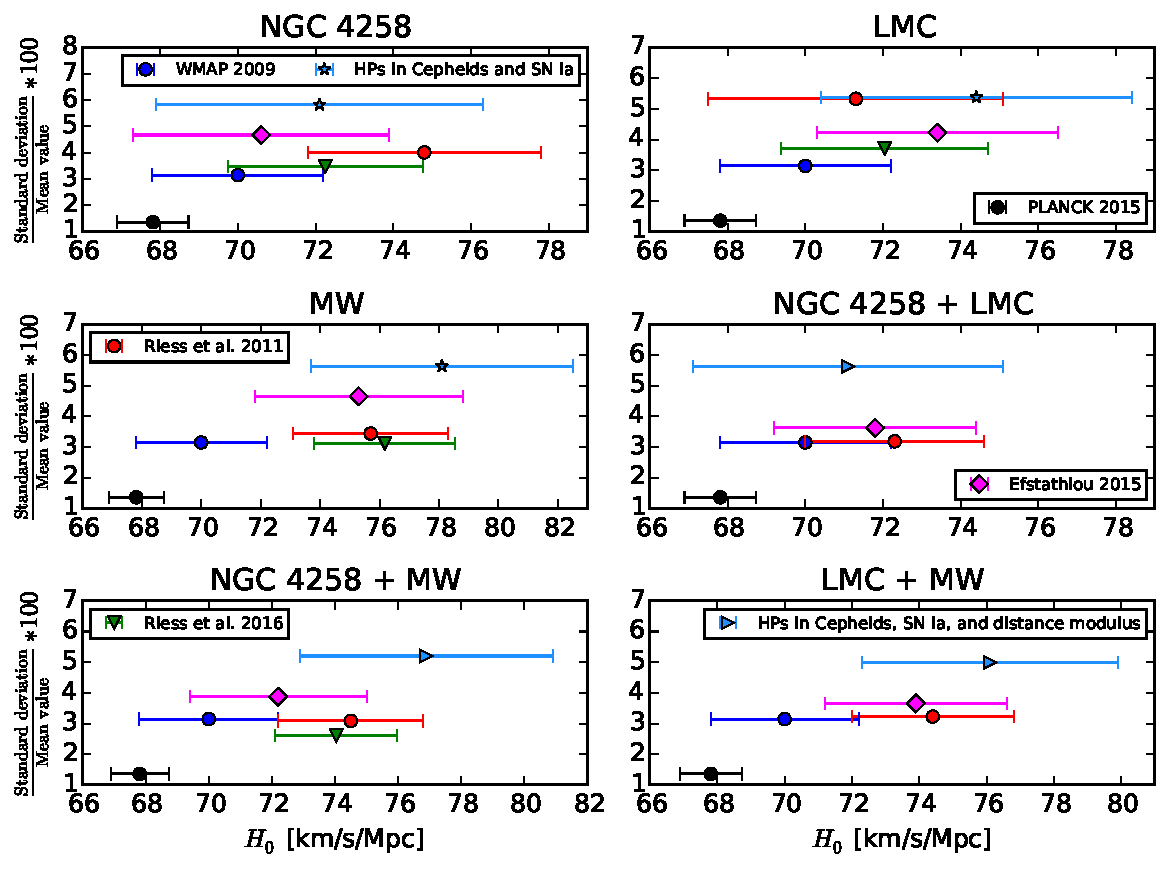
\includegraphics[scale=.8]{figures/chapter-h0/H0_values_anchor_combination.pdf}
\caption{Different measurements of the Hubble constant using different combinations of anchor distances. Colours and symbols are as in Figure \ref{Fig:H0-values-3-anchors}.}
\label{Fig:single-combined-anchor}
\end{figure}

\subsection{Megamaser system NGC 4258 distance modulus}
\label{Subsection:A-NGC4258}

In this subsection we apply our method to the sample of Cepheid variables and SNe Ia hosts in \cite{Riess:2011yx}, but restrict ourselves to a single anchor distance: the distance modulus to the megamaser system NGC 4258 from \cite{Humphreys:2013eja}. We include LMC Cepheid variables, but exclude MW Cepheid stars.  Results are shown in Table \ref{Table:NGC4258-fits}. We have explored two period cuts and two assumptions for the metallicity parameter $Z_W$.

The $H_0$ values in Table \ref{Table:NGC4258-fits} are shifted downwards w.r.t our 'standard analysis' value (Eq. \ref{Eq:H0-value-standard-analysis}) by $3-6 \%$. Fits with a tighter period cut prefer greater values of $H_0$: a $2\%$ change w.r.t those fits without period cut (independently of the metallicity dependence). Those changes are due to both $M_W-Z_W$ and $M_W-H_0$ degeneracies: a tighter period cut enhances metallicity dependence driving the Cepheid zero point to higher values which in turn prefers higher $H_0$. Allowing a metallicity dependence of the period-luminosity relation without prior on $Z_W$ we found a $>2\sigma$ departure from $Z_W=0$; This assumption, however, makes the Cepheid zero point $M_W$ less compatible with the value measured from MW Cepheid variables (see Eq. \eqref{Eq:MW-bestfit}). When HPs are used in Cepheid variables, SN Ia hosts, and distance modulus we obtain a $8\%$ measurement of the Hubble constant: the exclusion of two anchor distances in our 'standard analysis' makes the measurement more uncertain. Since for those fits the HP for the NGC 4258 distance modulus is always equal to one, we have also studied a couple of cases where only Cepheid variables and SNe Ia are included with HPs. As a result we obtain a $6\%$ measurement of $H_0$ which is still more uncertain than the corresponding case using the three anchor distances.

In the upper left panel of Figure \ref{Fig:single-combined-anchor} we show $H_0$ value from fit '$2^{ah}$' in Table \ref{Table:NGC4258-fits}, together with the values found by Riess et al. \cite{Riess:2011yx} ($H_0=74.8\pm 3.0 \, \km \second^{-1} \Mpc^{-1}$) which did not use the revised distance modulus from \cite{Humphreys:2013eja}, Efstathiou \cite{Efstathiou:2013via} ($H_0 = 70.6 \pm 3.3 \, \km \second^{-1} \Mpc^{-1}$), Riess et al. \cite{Riess:2016jrr} ($H_0=72.39\pm 2.56 \, \km \second^{-1} \Mpc^{-1}$) which used a redetermination of the distance modulus to NGC 4258. Our value is compatible with all previous direct determinations of $H_0$ and also with the indirect determinations from Planck and WMAP. The measurement using HPs is the most uncertain among the direct measurements due to inclusion of SNe Ia with HPs. The Planck collaboration used Efstathiou's value as a prior for $H_0$ when combining CMB measurements and local measurements of the Hubble constant. This assumption could lead to different conclusions in their analysis if another prior is utilised.

\begin{table}[tbp]
\centering
\begin{tabular}{@{}lccccr}
\hline
\multicolumn{6}{c}{NGC $4258$ anchor} \\
\hline
Fit & $H_0$ & $M_W$ & $b_W$ & $Z_W$ & $\sigma_{\intt}^{\LMC}$  \\
\hline
$1^a$ & $71.2\,(5.4)$& $-3.54\,(1.24)$ & $-3.15\,(0.06)\,[N]$ & $-0.285\,(0.140)\,[N]$ & $0.07$ \\
  
$1^b$ & $72.5\,(5.4)$& $-1.99\,(1.33)$ & $-3.25\,(0.05)\,[N]$ & $-0.457\,(0.150)\,[N]$ & $ 0.06$\\
   
$2^a$ & $71.1\,(5.5)$& $-6.00\,(0.22)$&$-3.17\,(0.06)\,[N]$ &$-0.006\,(0.020)\,[S]$ & $ 0.07$\\

$2^{ah}$ & $70.8\,(4.2)$& $-6.01\,(0.19)$&$-3.17\,(0.06)\,[N]$ &$-0.006\,(0.020)\,[S]$ & $ 0.07$\\

$2^b$ & $72.7\,(5.7)$& $-5.94\,(0.22)$&$-3.26\,(0.05)\,[N]$ &$-0.008\,(0.020)\,[S]$ & $ 0.06$\\

$2^{bh}$ & $72.1\,(4.2)$& $-5.95\,(0.19)$&$-3.26\,(0.05)\,[N]$ &$-0.008\,(0.020)\,[S]$ & $ 0.06$\\

\hline
\end{tabular}
\caption{\label{Table:NGC4258-fits} Numbers in brackets give the standard deviation. $[S]$ stands for the strong prior used in Subsection \ref{Subsection:combining-anchors}. SNe Ia hosts are included with HPs. Fits with superscript $^h$ include NGC 4258 distance modulus without HPs. For all the fits without superscript $^h$ the effective HP for the anchor is equal to one. Superscripts $^a$ and $^b$ indicate period cuts as in Table \ref{Table:LMC-fits}. For the SNe Ia hosts, $\sum_{i=1}^{8}  \alpha^{\eff,\,\SNe}_{i}$ ranges from $5.7$ (fits '$2^{ah}$' and '$2^a$') to $6.6$ (fit '$1^b$'). }
\end{table}


%\begin{table}[tbp]
%\centering
%\begin{tabular}{@{}lccccr}
%\hline
%\multicolumn{6}{c}{Distance parameters} \\
%\hline
%Host & SN Ia & $\mu_{0,i}-\mu_{0,4258}$ & $\mu_{0,i} $ best & $\alpha_{eff}$ & $\sigma_{int,i}^{R11}$\\
%\hline
%
% n4536 & SN 1981B & $1.619\,(0.0698)$&$31.04\,(0.12)$ &$1$ & $0.03$ \\
%
% n4639 & SN 1990N & $2.323\,(0.0844)$& $31.75\,(0.13)$& $1 $ & $0.01$\\
%
% n3370 & SN 1994ae & $2.502\,(0.0821)$& $31.93\,(0.13)$& $0.07 $ & $0.008$ \\
% 
% n3982 & SN 1998aq & $2.778\,(0.0656)$& $32.20\,(0.12)$& $ 0.04$ & $0.01$\\
%  
% n3021 & SN 1995al & $2.968\,(0.1080)$& $32.39\,(0.15)$& $ 0.6$ & $0.01$\\
%    
% n1309 & SN 2002fk & $3.229\,(0.0783)$& $32.65\,(0.13)$& $ 0.9$ & $0.01$\\
%
% n5584 & SN 2007af & $2.256\,(0.1009)$& $31.68\,(0.15)$& $ 0.09$ & $0.01$\\
%       
% n4038 & SN 2007sr & $2.379\,(0.0650)$& $31.80\,(0.12)$& $ 1$ & $0.01$\\
%       
%\hline
%\end{tabular}
%\caption{\label{Table:SNIa-NGC4258-fit-3} Numbers in brackets give the standard deviation on the parameters computed from the MCMC for fit $3^{ac}$ in Table \ref{Table:NGC4258-fits}. The last column gives the effective HP for each SN Ia.}
%\end{table}
%
%\begin{figure}[tbp]
%\centering % \begin{center}/\end{center} takes some additional vertical space
%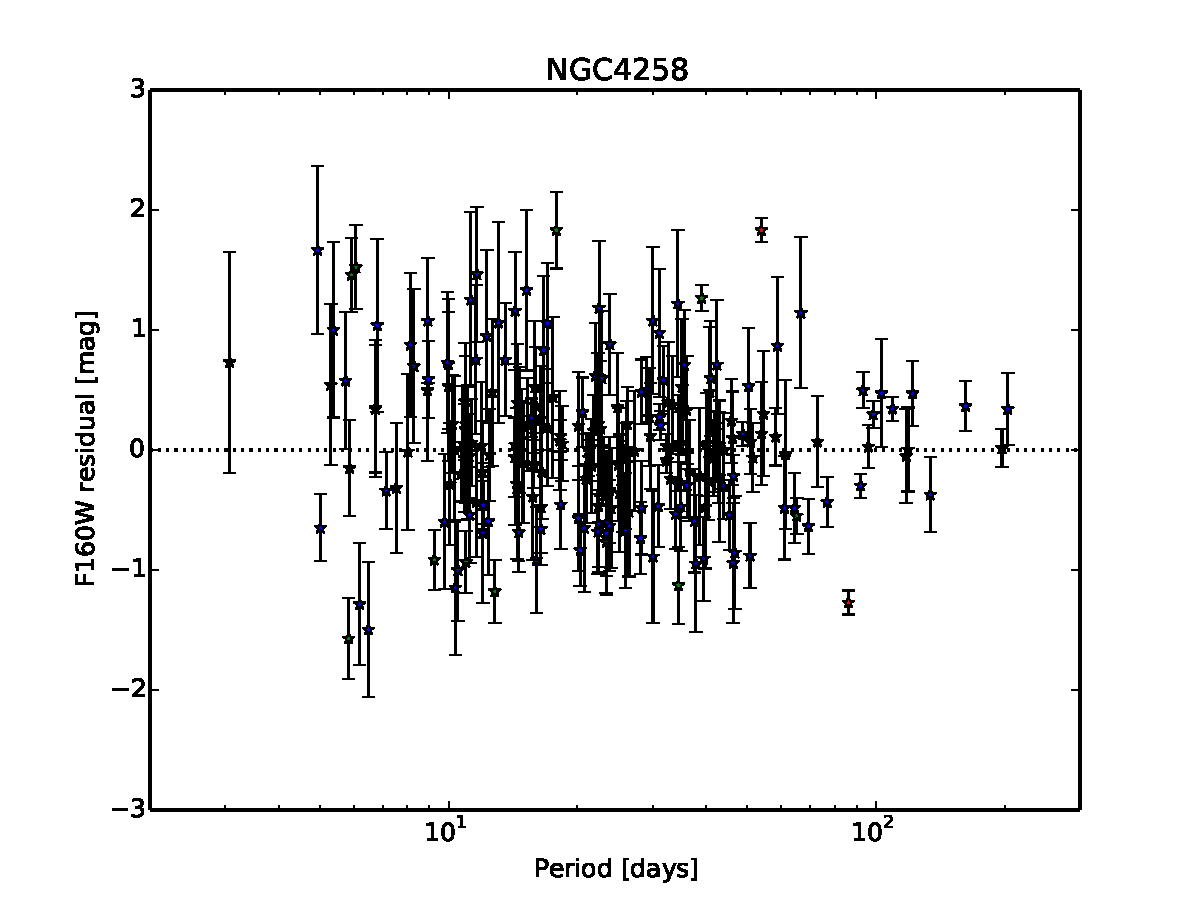
\includegraphics[scale=0.6]{effective_HP_F160W_cepheids_NGC4258.pdf}
%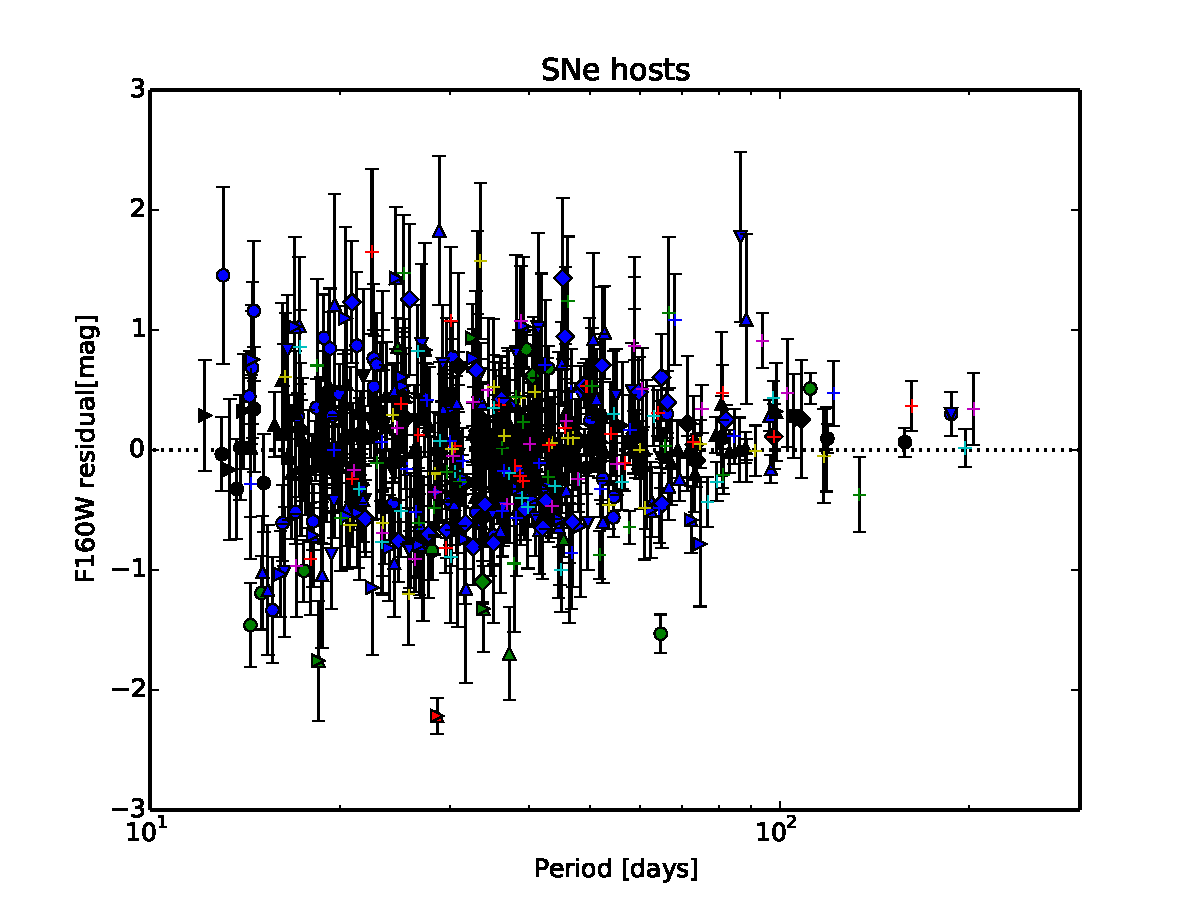
\includegraphics[scale=0.6]{effective_HP_F160W_cepheids_SNe.pdf} 
%\caption{Residuals for the P-L relation relative to global fit 3 in Table \ref{Table:NGC4258-fits}. Upper panel shows residuals for NGC4258 Cepheid variables and the SNe host galaxy Cepheid variables are shown in the bottom panel. Data points are colour-coded as in Figure \ref{Fig:LMC-Cepheid-variables-fit-c} corresponding to their HPs values. Error bars are not rescaled.}
%\label{Fig:Residuals-P-L-relation-fit-3}
%\end{figure}

\subsection{LMC distance modulus}
\label{Subsection:LMC-anchor}

In this subsection we apply our method to the sample of Cepheid variables and SNe Ia hosts in \cite{Riess:2011yx}, but restrict ourselves to a single anchor distance: the distance modulus to the LMC from \cite{Pietrzynski:2013gia}. We also include NGC4258 Cepheid variables, but omit MW Cepheid variables. Results are shown in Table \ref{Table:LMC-fits-anchor}. We have examined different period cuts and different assumptions for the metallicity dependence in the Leavitt Law.

The fits in Table \ref{Table:LMC-fits-anchor} show a $0-7\%$ shift in $H_0$ w.r.t the value in Eq. \eqref{Eq:H0-value-standard-analysis}. A period cut shifts $H_0$ values by $0.7-2\%$ (w.r.t. fits without period cut), whereas the use of HPs in LMC distance modulus changes $H_0$ values by $\lesssim 0.4\%$. In Figure \ref{Fig:constraints-fit-5a} we show $1-$D and $2-$D posteriors for fit '$5^a$'. Due to the $M_W-Z_W$, $M_W-H_0$, $Z_W-H_0$ degeneracies, $H_0$ is pushed towards higher values when a strong prior on the metallicity parameter $Z_W$ is utilised: the strong prior on $Z_W$ pushes $M_W$ to more negative values which in turn drives $H_0$ to higher values. When no prior on $Z_W$ is used along with a tighter cut period we observe a $3\sigma$ departure from $Z_W=0$. This, however, makes the Cepheid zero point $M_W$ less compatible with the value determined from MW Cepheid variables (Eq. \eqref{Eq:MW-bestfit}).

Fits in Table \ref{Table:LMC-fits-anchor} represent  $5-7\%$ measurements of the Hubble constant. In upper right panel of Figure \ref{Fig:single-combined-anchor} we show $H_0$ value of fit '$6^{ah}$' along with measurements by Riess et al. \cite{Riess:2011yx} ($H_0=71.3\pm 3.8 \, \km \second^{-1} \Mpc^{-1}$), Efstathiou \cite{Efstathiou:2013via} ($H_0 = 73.4 \pm 3.1 \, \km \second^{-1} \Mpc^{-1}$), Riess et al. \cite{Riess:2016jrr} ($H_0=71.93\pm 2.70 \, \km \second^{-1} \Mpc^{-1}$). Our measurement is almost as precise as that of \cite{Riess:2011yx} and is in good agreement with all the other direct determinations of the Hubble constant. While the WMAP value agrees at $1\sigma$ level with ours, the Planck value agrees at $2\sigma$ level.

\begin{table}[tbp]
\centering
\begin{tabular}{@{}lccccr}
\hline 
\multicolumn{6}{c}{LMC anchor} \\
\hline 
Fit & $H_0$ & $M_W$ & $b_W$ & $Z_W$ & $\sigma_{\intt}^{\LMC}$ \\
\hline
$5^a$ & $71.3\,(4.9)$& $-3.48\,(1.16)$ & $-3.15\,(0.06)\,[N]$& $-0.291\,(0.136)\,[N]$ & $0.07$ \\
 
$5^b$ & $70.1\,(4.5)$& $-2.11\,(1.28)$ & $-3.26\,(0.05)\,[N]$& $-0.450\,(0.150)\,[N]$ & $ 0.06$ \\	
  
$6^a$ & $74.5\,(4.9)$& $-5.90\,(0.20)$& $-3.17\,(0.06)\,[N]$& $-0.006\,(0.020)\,[S]$ & $0.07$ \\

$6^{ah}$ & $74.4\,(4.0)$& $-5.90\,(0.18)$& $-3.17\,(0.06)\,[N]$& $-0.006\,(0.020)\,[S]$& $0.07$ \\

$6^b$ & $75.0\,(4.8)$& $-5.87\,(0.20)$& $-3.26\,(0.05)\,[N]$& $-0.008\,(0.020)\,[S]$ & $ 0.06$ \\
   
$6^{bh}$ & $74.7\,(3.8)$& $-5.87\,(0.18)$& $-3.26\,(0.05)\,[N]$& $-0.008\,(0.020)\,[S]$& $ 0.06$ \\
   
\hline   
\end{tabular}
\caption{\label{Table:LMC-fits-anchor} Numbers in brackets give the standard deviation. $[S]$ stands for the strong prior used in Subsection \ref{Subsection:combining-anchors}. SNe Ia hosts are included with HPs. Fits with superscript $^h$ include LMC distance modulus without HPs. For all the fits without superscript $^h$ the effective HP for the anchor is equal to one. Superscripts $^a$ and $^b$ indicate period cuts as in Table \ref{Table:LMC-fits}. For SNe Ia hosts, $\sum_{i=1}^{8}  \alpha^{\eff,\,\SNe}_{i}$ ranges from $5.9$ (fit '$6^{bh}$') to $7$ (fit '$5^b$').}
\end{table}

\begin{figure}[hbtp]
\centering
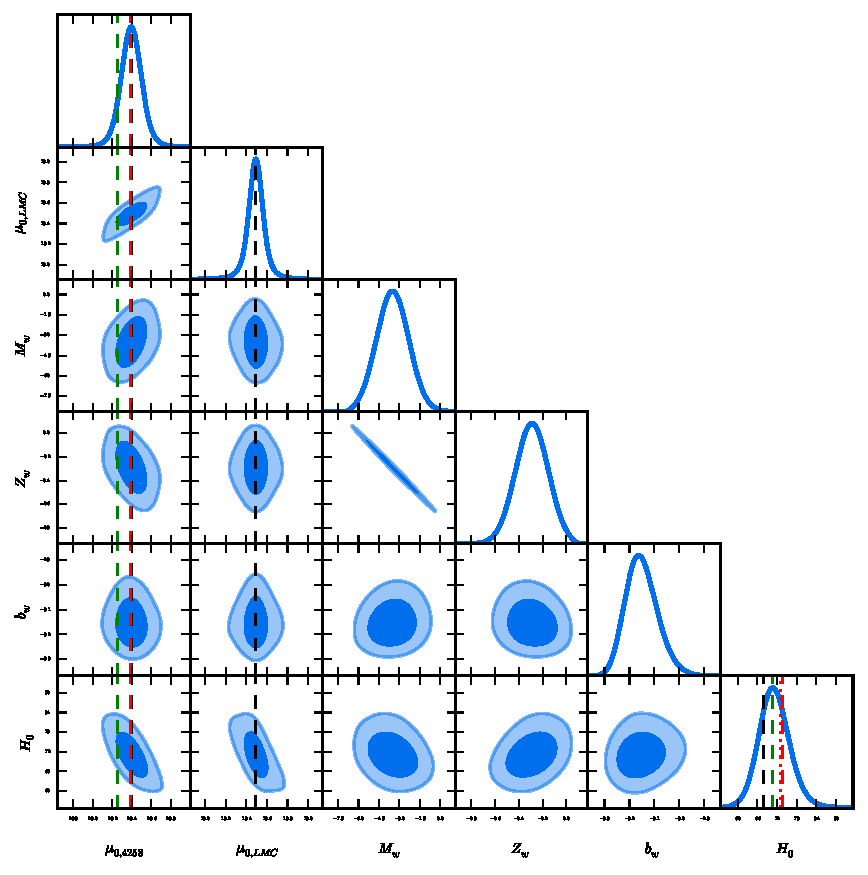
\includegraphics[scale=1]{figures/chapter-h0/triangle_figure_fit_5a.pdf}
\caption{Posterior constraints for fit '$5^a$'. Vertical lines show measurements of $\mu_{0,4258}$, $\mu_{0,\LMC}$, and $H_0$ as indicated in caption of Figure \ref{Fig:Main-analysis-fitM1a}.  \label{Fig:constraints-fit-5a}}
\end{figure}

\subsection{Parallax measurements of Cepheid variables in the Milky Way}
\label{Subsection:MW}

Parallax measurements of Cepheid variables (see Subsection \ref{Subsection:MW-1}) in our galaxy are used in this Section as the sole anchor distance scale. We include Cepheid variables in both the megamaser system NGC 4258 and those in the LMC. We show the resulting constraints in Table \ref{Table:MW-fits}. In addition to different period cuts and different assumptions for the metallicity dependence in the Leavitt Law, we have included some cases where those hosts galaxies whose slope $b_W$ departs from the LMC value (fit 'c' in Table \ref{Table:LMC-fits}) by $\gtrsim 2\sigma$ are excluded from the fit.

All fits in Table \ref{Table:MW-fits} including the whole data set are shifted upwards w.r.t our 'standard analysis' by $3-4\%$. In this case we obtain a $5-6\%$ measurement of the Hubble constant. A tighter period cut in the Leavitt Law shifts $H_0$ values by $0.3-0.4\%$ (w.r.t. fits without period cut). A strong prior on the metallicity parameter $Z_W$ drives downwards $H_0$ by $1-2\%$ (w.r.t. fits with no prior). When including the metallicity dependence without a prior we observe a slight $b_W-H_0$ degeneracy: less negative $b_W$ prefers higher $H_0$ values. Fits with a superscript $^l$ do not include Cepheid variables in galaxy hosts with a slope $b_W$ differing $\gtrsim 2\sigma$ from the LMC value. The main impact of this change is seen in $H_0$ having both mean value and standard deviation increased. Furthermore, those cases without prior on $Z_W$ present an enhancement on their metallicity dependence. As expected the slope $b_W$ is now closer to the LMC value (even without a tighter period cut).

In the middle left panel of Figure \ref{Fig:single-combined-anchor} we show $H_0$ value from fit $10^b$ along with values determined by Riess et al. \cite{Riess:2011yx} ($H_0=75.7\pm 2.6 \, \km \second^{-1} \Mpc^{-1}$); Efstathiou  \cite{Efstathiou:2013via} ($H_0 = 75.3 \pm 3.5 \, \km \second^{-1} \Mpc^{-1}$); Riess et al. \cite{Riess:2016jrr} ($H_0=76.09\pm 2.41 \, \km \second^{-1} \Mpc^{-1}$) that used a bigger sample of MW Cepheid variables. Our measurement is the most uncertain, but it is compatible with all other direct measurements showing that the value is robust against the statistical approach employed. All direct measurements present a $\approx 2\sigma$ disagreement with the Planck value.

\begin{table}[tbp]
\centering
\begin{tabular}{@{}lcccccr}
\hline 
\multicolumn{7}{c}{Milky Way anchor} \\
\hline 
Fit & $H_0$ & $M_W$ & $b_W$ & $Z_W$ & $\sigma_{\intt}^{\MW}$ & $\sigma_{\intt}^{\LMC}$ \\
\hline
$9^a$ & $78.1\,(4.4)$& $-3.44\,(1.25)$ & $-3.16\,(0.06)\,[N]$& $-0.272\,(0.140)\,[N]$ & $ 0.02 $ & $0.07$ \\

$9^{al}$ & $83.9\,(9.7)$& $-2.00\,(1.60)$ & $-3.27\,(0.05)\,[N]$& $-0.436\,(0.179)\,[N]$ & $ 0.02$ & $0.06$ \\
 
$9^b$ & $78.3\,(4.2)$& $-2.08\,(1.19)$ & $-3.26\,(0.05)\,[N]$& $-0.426\,(0.133)\,[N]$ & $0.02$ & $0.06$\\

$9^{bl}$ & $84.6\,(9.5)$& $-1.56\,(1.66)$ & $-3.27\,(0.05)\,[N]$& $-0.485\,(0.186)\,[N]$ & $0.02$ & $0.06$\\
  
$10^a$ & $77.4\,(4.4)$& $-5.81\,(0.18)$& $-3.17\,(0.06)\,[N]$& $-0.006\,(0.020)\,[S]$ & $0.02$ & $0.07$ \\

$10^{al}$ & $80.9\,(8.3)$& $-5.83\,(0.19)$& $-3.28\,(0.05)\,[N]$& $-0.007\,(0.020)\,[S]$ & $0.02$ & $0.06$ \\

$10^b$ & $77.1\,(4.1)$& $-5.81\,(0.18)$& $-3.26\,(0.05)\,[N]$& $-0.008\,(0.020)\,[S]$ & $0.02 $ & $0.06$ \\
   
$10^{bl}$ & $80.7\,(8.2)$& $-5.83\,(0.18)$& $-3.28\,(0.05)\,[N]$& $-0.006\,(0.020)\,[S]$ & $0.02 $ & $0.06$ \\
   
\hline   
\end{tabular}
\caption{\label{Table:MW-fits} For the MW Cepheid variables we find that $\sum_{i=1}^{13} \alpha^{\eff,\,\MW}_{i}$ ranges between $11.5$ (fit $9^a$) and $12$ (fit $10^b$). For the SNe Ia hosts the fit gives $\sum_{i=1}^{8} \alpha^{\eff,\,\SNe}_{i}$ ranging from $5.1$ (fit $10^a$) to $6.5$ (fit $9^a$).}
\end{table}

\subsection{Combining two distance anchors}
\label{Subsection-A-Combining-distance-anchors}

It is difficult to argue for specific choices of distance anchors, which is why we decided to combine all
anchors in the main text. Here we provide the constraints for different combinations of two anchor distances. Results are shown in Tables \ref{Table:Joint-Constraints-NGC-LMC}-\ref{Table:Joint-Constraints-LMC-MW}. 

Using distance moduli to both NGC 4258 and LMC as anchor distances we see that the effect of the strong prior on the metallicity parameter is less important than in the case where only LMC is utilised as anchor distance. There is also a $\approx 2\sigma$ departure from $Z_W=0$ when no prior on $Z_W$ is used, but the Cepheid zero point is is disagreement with the value measured by MW Cepheid variables alone. As noted before for the case using only LMC as anchor distance, again here the $M_W-H_0$, $M_W-Z_W$, and $Z_W-H_0$ degeneracies drive $H_0$ towards higher values. The change, however, is smaller than in the case where only LMC is used as anchor. In the middle right panel of Figure \ref{Fig:single-combined-anchor} we show $H_0$ value from fit '$14^b$' as well as the measurements of Riess et al. ($H_0=72.3\pm 2.3 \, \km \second^{-1} \Mpc^{-1}$) \cite{Riess:2011yx} and Efstathiou ($H_0=71.8\pm 2.6 \, \km \second^{-1} \Mpc^{-1}$) \cite{Efstathiou:2013via}.

Fits including both distance modulus to NGC 4258 and MW Cepheid variables as distance anchors follow same trend as fits only including MW Cepheid variables as distance anchor: $H_0$ is pushed downwards when a strong prior on the metallicity parameter is used, and the period cut does not have a big impact on the $H_0$ value. In the lower left panel of Figure \ref{Fig:single-combined-anchor} we show $H_0$ value from fit '$17^b$' as well as the measurements of Riess et al. ($H_0=74.5\pm 2.3 \, \km \second^{-1} \Mpc^{-1}$) \cite{Riess:2011yx}, Efstathiou ($H_0=72.2\pm 2.8 \, \km \second^{-1} \Mpc^{-1}$) \cite{Efstathiou:2013via}, and Riess et al ($H_0=73.85\pm 1.97 \, \km \second^{-1} \Mpc^{-1}$) \cite{Riess:2016jrr}.

Fits including both MW Cepheid variables and LMC distance modulus as anchor distances also follow same trend as for the case where MW Cepheid variables are used as the only anchor distance. In the lower right panel of Figure \ref{Fig:single-combined-anchor} we show measurement of fit '$22^b$' along with measurements by Riess et al. ($H_0=74.4\pm 2.4 \, \km \second^{-1} \Mpc^{-1}$) \cite{Riess:2011yx}, and Efstathiou ($H_0=73.9\pm 2.7 \, \km \second^{-1} \Mpc^{-1}$) \cite{Efstathiou:2013via}.
 
\begin{table}[tbp]
\centering
\begin{tabular}{@{}lccccr}
\hline
\multicolumn{6}{c}{NGC $4258\,+$ LMC anchors} \\
\hline
Fit & $H_0$ & $M_W$ & $b_W$ & $Z_W$  &$\sigma_{\intt}^{\LMC}$ \\
\hline 
$13^a$ &$ 71.1\,(4.0)$ & $-3.47\,(1.10)$& $-3.15\,(0.06)\,[N]$& $-0.293\,(0.128)\,[N]$ & $0.07$ \\

$13^b$ &$ 71.2\,(4.0)$ & $-2.27\,(1.16)$& $-3.25\,(0.05)\,[N]$& $-0.428\,(0.135)\,[N]$ & $0.06$ \\

$14^a$ &$73.0\,(4.1)$ & $-5.93\,(0.18)$& $-3.17\,(0.06)\,[N]$& $-0.007\,(0.020)\,[S]$ & $0.07$ \\

$14^b$ &$73.9\,(4.0)$ & $-5.89\,(0.18)$& $-3.26\,(0.05)\,[N]$& $-0.008\,(0.020)\,[S]$ & $0.06$ \\
\hline  
\end{tabular}
\caption{Distance modulus to both NGC 4258 and LMC are included with HPs. $\alpha_{\LMC}^{\eff}=\alpha_{4258}^{\eff}=1$ for all the fits except for the fit '$14^a$' where $\alpha_{4258}^{\eff}=0.7$. For the SNe Ia hosts the fits give $\sum_{i=1}^{8} \alpha^{\eff,\,\SNe}_{i}$ ranging from $5.4$ (fit $13^b$) to $6.5$ (fit $13^a$). \label{Table:Joint-Constraints-NGC-LMC} }
\end{table}

\begin{table}[tbp]
\centering
\begin{tabular}{@{}lcccccr}
\hline 
\multicolumn{7}{c}{NGC $4258\, +$ MW anchors} \\
\hline
Fit & $H_0$ & $M_W$ & $b_W$ & $Z_W$ &$\sigma_{\intt}^{\MW}$ & $\sigma_{\intt}^{\LMC}$ \\
\hline 
$17^a$ & $76.4\,(4.2)$&$-3.44\,(1.27)$ &$-3.18\,(0.06)\,[N]$ &$-0.277\,(0.142)\,[N]$ & $0.02$& $0.07$\\
 
$17^b$ & $76.9\,(4.0)$&$-2.13\,(1.27)$ &$-3.27\,(0.04)\,[N]$ &$-0.425\,(0.143)\,[N]$ & $0.01$& $0.06$\\
 
$18^a$ &$75.6\,(4.2)$ &$-5.85\,(0.18)$ &$-3.20\,(0.05)\,[N]$ &$-0.006\,(0.020)\,[S]$ &$0.02$ & $0.06$\\

$18^b$ &$75.8\,(3.9)$ &$-5.84\,(0.18)$ &$-3.27\,(0.04)\,[N]$ &$-0.008\,(0.020)\,[S]$ &$0.02$ & $0.06$\\
\hline  
\end{tabular}
\caption{Distance modulus to the megamaser system NGC 4258 is included with HPs. All the fits have $\alpha_{4258}^{\eff}<1$, values ranging from $0.2$ (fit '$17^a$') to $0.5$ (fit '$17^b$'). For the SNe Ia hosts the fits give $\sum_{i=1}^{8} \alpha^{\eff,\,\SNe}_{i}$ ranging from $5.6$ (fit $17^b$) to $6.4$ (fit $17^a$) \label{Table:Joint-Constraints-NGC-MW} }
\end{table}

\begin{table}[tbp]
\centering
\begin{tabular}{@{}lcccccr}
\hline
\multicolumn{7}{c}{LMC $+$ MW anchors} \\
\hline
Fit & $H_0$ & $M_W$ & $b_W$ & $Z_W$ &$\sigma_{\intt}^{\LMC}$ & $\sigma_{\intt}^{\MW}$ \\
\hline 
$21^a$ & $76.0\,(4.2)$ &$-4.33\,(1.16)$ &$-3.18\,(0.06)\,[N]$ &$-0.178\,(0.131)\,[N]$ & $0.07$& $0.02$\\

$21^b$ & $76.2\,(4.1)$ &$-3.10\,(1.31)$ &$-3.27\,(0.05)\,[N]$ &$-0.318\,(0.147)\,[N]$ & $0.06$& $0.02$\\
 
$22^a$ &$76.0\,(4.0)$ &$-5.86\,(0.18)$ &$-3.19\,(0.05)\,[N]$ &$-0.004\,(0.020)\,[S]$ & $0.06$ & $0.02$\\

$22^b$ &$76.1\,(3.8)$ &$-5.84\,(0.18)$ &$-3.27\,(0.04)\,[N]$ &$-0.007\,(0.020)\,[S]$ &$0.06$ & $0.02$\\
\hline 
\end{tabular}
\caption{Both SNe Ia and distance modulus to LMC are included with HPs. Fit '$22^b$' is the only one for which the distance modulus to LMC is not down-weighted; Values for the others fits range from $0.1$ (fits '$21^a$' and '$21^b$') to $0.6$ (fit '$22^a$'). For the SNe Ia hosts the fits give $\sum_{i=1}^{8} \alpha^{\eff,\,\SNe}_{i}$ ranging from $5.7$ (fit $22^b$) to $6.6$ (fit $22^b$). The sum of effective HPs for MW Cepheid variables ranges from $11.7$ (fits '$21^b$' and '$22^b$') to $12.1$ (fit '$21^a$').\label{Table:Joint-Constraints-LMC-MW}}
\end{table}
%\begin{tabular}{@{}lcccccr}
%\hline 
%\multicolumn{7}{c}{NGC $4258 +$ LMC $+$ MW anchors} \\
%\hline
%Fit & $H_0$ & $M_W$ & $b_W$ & $Z_W$ &$\sigma_{\intt}^{\LMC}$ & $\sigma_{\intt}^{\MW}$ \\
%\hline 
%$25^a$ & $74.8\,(4.0)$&$-4.33\,(1.10)$ &$-3.19\,(0.05)\,[N]$ &$-0.180\,(0.124)\,[N]$ & $0.06$& $0.009$& $0.03$ \\

%$25^b$ & $75.1\,(3.9)$&$-3.19\,(1.24)$ &$-3.28\,(0.04)\,[N]$ &$-0.310\,(0.140)\,[N]$ & $0.06$& $0.009$& $0.01$ \\

%$26^a$ & $74.6\,(3.9)$&$-5.88\,(0.18)$ &$-3.19\,(0.05)\,[N]$ &$-0.005\,(0.020)\,[Y]$ & $0.06$& $0.011$& $0.04$\\

%$26^b$ & $75.5\,(3.9)$&$-5.86\,(0.18)$ &$-3.27\,(0.04)\,[N]$ &$-0.007\,(0.020)\,[Y]$ & $0.06$& $0.008$& $0.01$\\

%$27^a$ & $75.2\,(3.9)$&$-5.86\,(0.18)$ &$-3.22\,(0.04)\,[Y]$ &$-0.004\,(0.020)\,[Y]$ & $0.06$& $0.009$& $0.03$\\

%$27^b$ & $75.9\,(3.8)$&$-5.84\,(0.18)$ &$-3.28\,(0.04)\,[Y]$ &$-0.006\,(0.020)\,[Y]$ & $0.05$& $0.009$& $0.01$\\

%$28^a$ & $75.0\,(4.0)$&$-4.47\,(1.13)$ &$-3.22\,(0.04)\,[Y]$ &$-0.162\,(0.127)\,[N]$ &$0.06$ &$0.009$ & $0.03$\\
  
%$28^b$ & $75.9\,(4.0)$&$-3.22\,(1.29)$ &$-3.28\,(0.04)\,[Y]$ &$-0.304\,(0.145)\,[N]$ & $0.05$& $0.009$& $0.01$\\
  
%\hline 
%\end{tabular}


%\subsection{Previous Results}
%\label{Section:Results}
%
%Table \ref{Table:Constraints} shows previous results with fixed $\sigma_{\rm int}$. \commentr{Constraints on relevant parameters. Fits with $\star$ include anchors with HPs and those with $\diamond$ include HPs in SNIa.$\heartsuit$ includes HPs in metallicity. $\square$ includes MW dataset with a HP with Jeffrey's prior.}
%
%\begin{table}[tbp]
%\centering
%\begin{tabular}{@{}lcccccccr}
%\hline
%\multicolumn{9}{c}{NGC $4258$ anchor} \\
%\hline
%Fit & $H_0$ & $zp_W$ & $b_W$ & $Z_W$ & $\sigma_{int}$ & Prior $Z_W$ & Prior $b_W$  & P \\
%\hline
% A1 & $70.5\,(3.1)$& $26.34\,(0.26)$ & $-3.00\,(0.13)$ & $-0.008\,(0.020)$& $0.14$ & S & N & $60$ \\
%  
% A2 & $71.2\,(3.3)$& $26.32\,(0.26)$&$-2.99\,(0.14)$ &$-0.007\,(0.020)$ & $0.2$ & S & N & $60$ \\
%
% A3 & $70.3\,(2.9)$& $26.12\,(0.22)$& $-2.86\,(0.09)$& $-0.006\,(0.020)$& $0.2$ & S & N & $205$ \\
% 
%\end{tabular}
%\begin{tabular}{@{}lcccccccr}
%\hline 
%\multicolumn{9}{c}{LMC anchor} \\
%\hline 
%Fit & $H_0$ & $zp_W$ & $b_W$ & $Z_W$ & $\sigma_{int}$ & Prior $Z_W$ & Prior $b_W$  & P \\
%\hline
% A4 & $70.0\,(2.5)$& $19.35\,(1.31)$ & $-3.19\,(0.07)$& $-0.43\,(0.15)$& $0.14$ & N & N & $60$ \\
% 
% A5 & $70.2\,(2.9)$& $19.30\,(1.42)$& $-3.19\,(0.07)$& $-0.42\,(0.17)$& $0.2$ & N & N & $60$ \\
% 
% A6 & $70.4\,(2.0)$& $18.36\,(1.20)$ & $-3.07\,(0.07)$& $-0.32\,(0.14)$& $0.2$ & N & N & $205$ \\
% 
% A7 & $73.9\,(2.6)$& $15.80\,(0.19)$ & $-3.20\,(0.07)$& $-0.006\,(0.020)$& $0.14$ & S & N & $60$ \\
% 
% A8 & $72.8\,(2.3)$& $15.82\,(0.19)$& $-3.22\,(0.07)$& $-0.006\,(0.020)$& $0.2$ & S & N & $60$ \\
% 
% A9 & $73.9\,(2.7)$& $15.66\,(0.19)$ & $-3.09\,(0.07)$& $-0.005\,(0.020)$& $0.2$ & S & N & $205$ \\
%   
%\end{tabular}
%\begin{tabular}{@{}lcccccccr}
%\hline
%\multicolumn{9}{c}{MW anchor} \\
%\hline 
%Fit & $H_0$ & $M_W$ & $b_W$ & $Z_W$ & $\sigma_{int}$ & Prior $Z_W$ & Prior $b_W$  & P \\
%\hline
%A10 & $81.5\,(4.5)$& $-5.74\,(0.19)$& $-3.06\,(0.12)$ & $-0.007\,(0.020)$ & $0.14$ & S & N & $60$ \\
% 
%A11 &$80.1\,(4.7)$ & $-5.76\,(0.19)$ &$-3.09\,(0.13)$ & $-0.006\,(0.020)$& $0.2$ & S & N & $60$ \\
% 
%A12 & $85.0\,(4.2)$ & $-5.72\,(0.19)$ &$-2.90\,(0.09)$ & $-0.006\,(0.020)$& $0.2$ & S & N & $205$ \\
% 
%\end{tabular}
%\begin{tabular}{@{}lcccccccr}
%\hline
%\multicolumn{9}{c}{NGC $4258+$ LMC anchors} \\
%\hline
%Fit & $H_0$ & $M_W$ & $b_W$ & $Z_W$ & $\sigma_{int}$ & Prior $Z_W$ & Prior $b_W$  & P \\
%\hline 
%A13 &$72.6\,(1.7)$ & $-5.90\,(0.17)$& $-3.21\,(0.07)$& $-0.008\,(0.020)$& $0.14$ & S & N & $60$ \\
%
%A13$\heartsuit$ &$72.6\,(2.8)$ & $-5.66\,(0.42)$& $-3.21\,(0.07)$& $-0.037\,(0.049)$& $0.14$ & S & N & $60$ \\
% 
%A14 & $72.1\,(2.4)$ & $-5.91\,(0.18)$&$-3.22\,(0.07)$ &$-0.008\,(0.020)$ & $0.2$ & S & N & $60$ \\
%
%A14$\star$ & $72.1\,(2.9)$ & $-5.92\,(0.19)$ & $-3.21\,(0.07)$ & $-0.007\,(0.020)$ & $0.2$ & S & N & $60$ \\
%
%A14$\diamond$ & $74.1\,(3.9)$ & $-5.91\,(0.18)$ & $-3.22\,(0.07)$ & $-0.007\,(0.020)$ & $0.2$ & S & N & $60$ \\
% 
%A14$\star\diamond$ & $74.2\,(4.1)$ & $-5.93\,(0.18)$ & $-3.22\,(0.07)$ & $-0.006\,(0.020)$ & $0.2$ & S & N & $60$ \\
% 
%A15 &$72.3\,(2.4)$ &$-5.94\,(0.18)$ &$-3.10\,(0.07)$ &$-0.007\,(0.020)$ & $0.2$ & S & N & $205$ \\
% 
%A15$\star$ & $72.3\,(3.0)$ & $-5.96\,(0.19)$ & $-3.10\,(0.07)$ & $-0.006\,(0.020)$ & $0.2$ & S & N & $205$ \\
% 
%\end{tabular}
%\begin{tabular}{@{}lcccccccr}
%\hline 
%\multicolumn{9}{c}{NGC $4258 +$ MW anchors} \\
%\hline
%Fit & $H_0$ & $M_W$ & $b_W$ & $Z_W$ & $\sigma_{int}$ & Prior $Z_W$ & Prior $b_W$  & P \\
%\hline 
%A16 & $74.1\,(3.0)$&$-5.87\,(0.18)$ &$-3.21\,(0.10)$ &$-0.006\,(0.020)$ & $0.14$ & S & N & $60$ \\
% 
%A17 &$74.8\,(2.8)$ &$-5.85\,(0.18)$ &$-3.21\,(0.11)$ &$-0.007\,(0.019)$ & $0.2$ & S & N & $60$ \\
% 
%A18 &$76.1\,(3.0)$ &$-5.90\,(0.19)$ &$-3.03\,(0.08)$ &$-0.005\,(0.020)$ & $0.2$ & S & N & $205$ \\
% 
%\end{tabular}
%\begin{tabular}{@{}lcccccccr}
%\hline
%\multicolumn{9}{c}{LMC $+$ MW anchors} \\
%\hline
%Fit & $H_0$ & $M_W$ & $b_W$ & $Z_W$ & $\sigma_{int}$ & Prior $Z_W$ & Prior $b_W$  & P \\
%\hline 
%A19 & $74.7\,(2.5)$ &$-5.86\,(0.18)$ &$-3.23\,(0.07)$ &$-0.005\,(0.020)$ & $0.14$ & S & N & $60$ \\
% 
%A20 &$74.7\,(2.5)$ &$-5.86\,(0.18)$ &$-3.24\,(0.07)$ &$-0.004\,(0.020)$ & $0.2$ & S & N & $60$ \\
% 
%A21 &$75.2\,(2.6)$ &$-5.89\,(0.18)$ &$-3.13\,(0.06)$ &$-0.002\,(0.020)$ & $0.2$ & S & N & $205$ \\
% 
%\end{tabular}
%\begin{tabular}{@{}lcccccccr}
%\hline 
%\multicolumn{9}{c}{NGC $4258 +$ LMC $+$ MW anchors} \\
%\hline
%Fit & $H_0$ & $M_W$ & $b_W$ & $Z_W$ & $\sigma_{int}$ & Prior $Z_W$ & Prior $b_W$  & P \\
%\hline 
%A22 & $72.3\,(2.1)$&$-5.89\,(0.17)$ &$-3.27\,(0.06)$ &$-0.006\,(0.020)$ & $0.14$ & S & N & $60$ \\
%
%A22$\star$ & $73.9\,(2.6)$&$-5.86\,(0.18)$ &$-3.25\,(0.07)$ &$-0.006\,(0.020)$ & $0.14$ & S & N & $60$ \\
%
%A22$\diamond$ & $75.4\,(3.2)$&$-5.88\,(0.18)$ &$-3.26\,(0.06)$ &$-0.005\,(0.020)$ & $0.14$ & S & N & $60$ \\
%
%A22$\star \diamond$ & $76.4\,(3.8)$&$-5.86\,(0.18)$ &$-3.25\,(0.07)$ &$-0.006\,(0.020)$ & $0.14$ & S & N & $60$ \\
% 
%A23 & $72.5\,(2.6)$&$-5.88\,(0.18)$ &$-3.27\,(0.07)$ &$-0.006\,(0.020)$ & $0.2$ & S & N & $60$ \\
% 
%A23$\star$ & $73.9\,(2.7)$&$-5.87\,(0.18)$ &$-3.25\,(0.07)$ &$-0.005\,(0.020)$ & $0.2$ & S & N & $60$ \\
%
%A23$\diamond$ & $74.0\,(2.1)$&$-5.89\,(0.18)$ &$-3.27\,(0.06)$ &$-0.005\,(0.020)$ & $0.2$ & S & N & $60$ \\
%
%A23$\star \diamond$ & $76.4\,(3.4)$&$-5.86\,(0.18)$ &$-3.25\,(0.07)$ &$-0.005\,(0.020)$ & $0.2$ & S & N & $60$ \\
% 
%A23$\square$ & $73.6\,(2.3)$&$-5.86\,(0.18)$ &$-3.30\,(0.06)$ &$-0.004\,(0.020)$ & $0.2$ & S & N & $60$ \\
% 
%A24 &$71.2\,(1.4)$ &$-5.91\,(0.18)$ &$-3.18\,(0.06)$ &$-0.005\,(0.020)$ & $0.2$ & S & N & $205$ \\
% 
%A24$\star$ &$74.7\,(2.8)$ &$-5.88\,(0.18)$ &$-3.14\,(0.06)$ &$-0.003\,(0.020)$ & $0.2$ & S & N & $205$ \\
%
%A24$\diamond$ &$75.1\,(3.9)$ &$-5.91\,(0.18)$ &$-3.16\,(0.06)$ &$-0.004\,(0.020)$ & $0.2$ & S & N & $205$ \\
%
%A24$\star \diamond$ &$76.5\,(4.2)$ &$-5.88\,(0.18)$ &$-3.15\,(0.06)$ &$-0.003\,(0.020)$ & $0.2$ & S & N & $205$ \\
% 
% 
%\hline 
%\end{tabular}
%\caption{\label{Table:Constraints} Constraints on relevant parameters. Fits with $\star$ include anchors with HPs and those with $\diamond$ include HPs in SNIa.$\heartsuit$ includes HPs in metallicity. $\square$ includes MW dataset with a HP with Jeffrey's prior.}
%\end{table}


%\begin{figure}[tbp]
%\centering % \begin{center}/\end{center} takes some additional vertical space
%\includegraphics[scale=0.75]{effective_HP_cepheids_Efstathiou.pdf} 
%\caption{P-L magnitude residuals relative to  Plot with hyper-parameters and data points.}
%\label{Fig:hyper-parameters-and-data}
%\end{figure}


%\begin{figure}
%
%\caption{\label{Fig:H0-posteior} Posterior of $H_0$ when adding different terms and data.}
%\end{figure}
